\input{preamble.txt}
\usepackage{vwcol}
\begin{document}

\section{Introduction to Java}
\begin{itemize}

	\item What is Java?
	\begin{itemize}
		\item An object-oriented language invented by James Gosling in 1994 at Sun Microsystems
		\item Write once, run anywhere (WORA)
		\item Widely-used in industry
		\item Used to develop software running on:
		%				\begin{itemize}
		%					\item Desktop Computers
		%					\item Servers
		%					\item Mobile devices
		%				\end{itemize}
		\begin{itemize}
			\begin{minipage}[t]{0.25\textwidth}
				\item Desktop Computers
			\end{minipage}
			\begin{minipage}[t]{0.15\textwidth}
				\item Servers
			\end{minipage}
			\begin{minipage}[t]{0.2\textwidth}
				\item Mobile devices
			\end{minipage}
		\end{itemize}
	\end{itemize}

	\item Java Programs
	\begin{enumerate}
		\item Writing the source code using a text editor
		\item Translating the source code into Java bytecode using a compiler
		\begin{itemize}
			\item Bytecode is similar to machine instructions but is architecture neutral and can run on any platform that has a Java Virtual Machine (JVM)
		\end{itemize}
		\item Executing the bytecode
		\begin{itemize}
			\item The JVM is an interpreter: it translates bytecode into the target machine language code one at a time rather than the whole program as a single unit
			\item Each step is executed immediately after it is translated\\[-21pt]
		\end{itemize}
	\end{enumerate}
	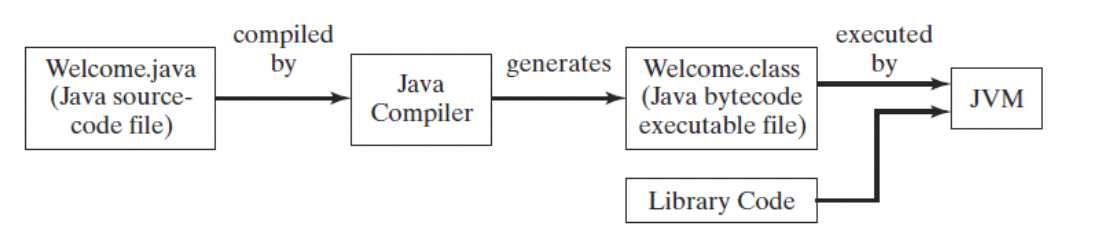
\includegraphics[scale=.75]{Compile flow.png}\\[-30pt]

	\item Integrated Development Environment
	\begin{itemize}
		\item A system comprising several tools that facilitate software development and testing
		\item Popular IDEs:
		\begin{itemize}
			\begin{minipage}[t]{0.15\textwidth}
				\item Eclipse
			\end{minipage}
			\begin{minipage}[t]{0.15\textwidth}
				\item NetBeans
			\end{minipage}
			\begin{minipage}[t]{0.2\textwidth}
				\item IntelliJ
			\end{minipage}
		\end{itemize}
	\end{itemize}

	\item Data Types
	\begin{itemize}
		\item Eight primitive types
		\begin{itemize}
			\item byte, char, short, int, long, float, double, boolean
		\end{itemize}
		\item Objects
		\begin{itemize}
			\item Defined using \textbf{classes}
			\item Java provides wrapper classes to use primitive types as objects (e.g. Integer, Double, etc)
		\end{itemize}
	\end{itemize}

	\item Numeric Primitive Types
	%	\includegraphics[scale=.7]{Primitive types.png}
	\begin{center}
		\begin{tabular}{ l l l }
			\hline
			\textit{Name} & \textit{Range} & \textit{Storage Size}\\
			\hline\\[-10pt]
			\textbf{byte} & $ -2^7 $ to $ 2^7 - 1 \, (-128 \text{ to } 127)  $  & 8-bit signed\\
			\textbf{short} & $ -2^{15} $ to $ 2^{15} - 1 \, (-32768 \text{ to } 32767)  $ & 16-bit signed\\
			\textbf{int} & $ -2^{31} $ to $ 2^{31} - 1 \, (-2147483648 \text{ to } 2147483647)  $ & 32-bit signed\\
			\textbf{long} & $ -2^{63} $ to $ 2^{63} - 1  $ & 64-bit signed\\
			& (i.e., $-9223372036854775808 \text{ to } 9223372036854775807$) & \\
			\textbf{float} & Negative range: $ -3.4028235\text{E} + 38$ to $ -1.4\text{E} -45$ & 32-bit IEEE 754\\
			& Positive range: $ 1.4\text{E} -45 $ to $ 3.4028235\text{E} + 38 $ & \\
			\textbf{double} & Negative range: $ -1.7976931348623137\text{E} + 38$ to $ -4.9\text{E} - 324$ & 64-bit IEEE 754\\
			& Positive range: $4.9\text{E} - 324$ to $1.7976931348623137\text{E} + 38$ &
		\end{tabular}
	\end{center}

	\item Classes
	\begin{itemize}
		\item A typical Java class includes the following:
		\begin{itemize}
			\item Data fields to represent the state of an object
			\item Methods to represent the behavior of an object. Each method has:
			\begin{itemize}
				\item A return type (\textbf{void} if nothing is returned)
				\item Zero or more arguments
			\end{itemize}
			\item Special type of methods, known as constructors, that perform initialization actions. A constructor:
			\begin{itemize}
				\item Has no return type (not even \textbf{void})
				\item Has zero or more arguments
				\item Should have the same name as the class
				\item Is invoked using the \textbf{new} operator
			\end{itemize}
		\end{itemize}
		\item Instantiation is creating an object (or an instance of a class)
	\end{itemize}

	\item The \textit{main} method
	\begin{itemize}
		\item The main method is the entry point where the program begins
		execution
		\item Should have the following form:
		\begin{Verbatim}
			public static void main(String [] args) {
				//write your code here
			}
		\end{Verbatim}
	\end{itemize}

	\item Default values
	\begin{itemize}
		\item The default value of a data field is:
		\begin{itemize}
			\begin{minipage}[t]{0.25\textwidth}
				\item \textbf{\textit{null}} for a reference type
			\end{minipage}
			\begin{minipage}[t]{0.25\textwidth}
				\item \textbf{0} for a numeric type
			\end{minipage}

			\begin{minipage}[t]{0.25\textwidth}
				\item \textbf{false} for a boolean type
			\end{minipage}
			\begin{minipage}[t]{0.25\textwidth}
				\item \textbf{`$\backslash$u0000'} for a char type
			\end{minipage}
		\end{itemize}
		\item Java assigns no default value to a local variable inside a method
	\end{itemize}

	\item Scope
	\begin{itemize}
		\item The scope of fields and methods is the entire class
		\item The scope of a local variable starts from its declaration until the end
		of the block that contains it
	\end{itemize}

	\item Differences between Variables of Primitive Types and Reference Types
	\begin{itemize}
		\item Every variable represents a memory location that holds a value
		\item For a variable of a primitive type, the value is of the primitive type
		\item For a variable of a reference type, the value is a reference to where an object is located (i.e. a pointer)
		\item When you assign one variable to another:
		\begin{itemize}
			\item For a variable of a primitive type, the real value of one variable is assigned to
			the other variable
			\item For a variable of a reference type, the reference of one variable is assigned to the other variable.
		\end{itemize}
	\end{itemize}

	\item The \textit{this} reference
	\begin{itemize}
		\item The \textbf{this} \textit{keyword} is the name of a reference that an object can use to
		refer to itself
		\item It can be used to reference the object’s instance members
	\end{itemize}

	\item The \textit{static} modifier
	\begin{itemize}
		\item Static fields/methods can be accessed from a reference variable or
		from their class name
		\item Non-static (or instance) fields/methods can only be accessed from a reference variable
	\end{itemize}

	\item Arrays
	\begin{itemize}
		\item An array is a data structure that represents a collection of the same types of data
		\item Once an array is created, its size is fixed
		\begin{itemize}
			\item e.g. \textbf{int [] A = new int[10];}
		\end{itemize}
		\item The size of an array A can be found using \textbf{A.length}
		\item When an array is created, its elements are assigned the default value
		\item Array elements could be initialized individually
		\begin{itemize}
			\item e.g. \textbf{A[0] = 5;}
		\end{itemize}
		\item Array initializer (combines declaration, creation, and initialization)
		\begin{itemize}
			\item e.g. \textbf{double[] myList = {1.9, 2.9, 3.4, 3.5};}
		\end{itemize}
	\end{itemize}

	\item Two-dimensional Arrays
	\begin{itemize}
		\item The syntax for declaring a two-dimensional array is:
		\begin{itemize}
			\item \textbf{elementType [][] arrayRefVar;} (e.g. \textbf{int[][] matrix;})
		\end{itemize}
		\item For a two-dimensional array A, \textbf{A.length} returns the number of rows
		\item Two-dimensional array examples:\\
		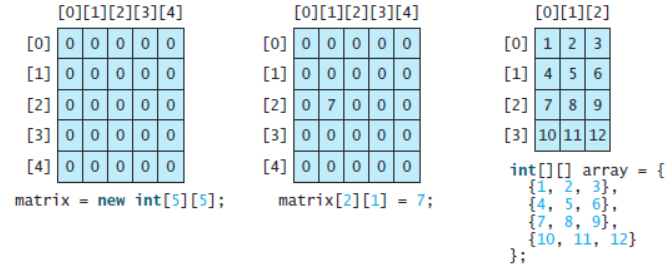
\includegraphics[scale=0.9]{array.png}
	\end{itemize}
\end{itemize}
\end{document}